\input{01-EtudeAeronefs/img/Cycle4Temps/ElementsMoteur.tex}

\section{Les groupes motopropulseurs}

	\subsection{Moteurs à pistons}
		\subsubsection{Description du moteur à piston}
		Le moteur à piston, également appelé moteur à combustion interne ou moteur à explosion est un moteur qui transforme l'énergie chimique contenue dans le carburant (essence, gasoil, gaz...) en énergie mécanique.
		\begin{figure}[H]
  		\centering
    		% INTAKE STROKE
\begin{tikzpicture}[scale=\echelleTikz]
  \def\d{-60}
  \engine{10};
  \draw[vector] (\d:.6*\R) arc (\d:\d-80:.55*\R);
  \fill[\gas]
    (VLo) to[out=110,in=0] ++ (-1.5,0.6) -- ($(VLo)+(-1.5,1.3)$) to[out=0,in=110] (VLm) to[out=\vl-90,in=\vl-90] cycle;
  \wall
  \valveL{.3}
  \valveR{.1}
  
  \draw[arrow] (VL) ++ (-.2,.2) --++ (-1,-.5)
    node[below left=-2,align=right,scale=1.4] {valve\\[-2pt]d'admission};
  \draw[arrow] (VR) ++ (.2,.1) --++ (1,-.5)
    node[below right=-2,align=left,scale=1.4] {valve\\[-2pt]d'échappement};
  \draw[arrow] (O) ++ (-.2,.4) --++ (-2.0,.9)
    node[left=-20,above left=2,scale=1.4] {villebrequin};
  \draw[arrow] (P) ++ (1.1,-.2) --++ (1.2,-.5)
    node[below right=-2,scale=1.4] {piston};
  \draw[arrow] (P) ++ (1.5,0.4) --++ (1.2,-.5)
    node[below right=-2,scale=1.4] {cylindre};
  \draw[arrow] (P) ++ (-1,0.97) --++ (-1.2,-.5);
  \draw[arrow] (P) ++ (-1,0.67) --++ (-1.2,-.2) %-0.5 - (0.97-0.67) = -0.2
    node[below left=-2,scale=1.4] {segments};
  \draw[arrow] (PL) ++ (2.2,-1.9) --++ (1.68,-.7)
    node[below right=-2,scale=1.4] {bielle};
  \draw[arrow] (O) ++ (-1.9,-0.8) --++ (-1.2,.5)
    node[left=-20,above left=2,scale=1.4] {carter};
  \draw[arrow] (S) ++ (150:.2) --++ (-.5,.7)
    node[above=-1,align=center,scale=1.4] {bougie};
  \draw[arrow] (VLm) ++ (-1.5,.5) --++ (-1.5,.7)
    node[above left=-2,align=right,scale=1.4] {pipe\\[-2pt]d'admission};
  \draw[arrow] (VRm) ++ (1.5,.5) --++ (1.5,.7)
    node[above right=-2,align=left,scale=1.4] {pipe\\[-2pt]d'échappement};
  
\end{tikzpicture}
  		\legende{Schéma d'un moteur à piston}{tikz::schemaMoteurPiston}
		\end{figure}
		
		Le moteur à piston est composé des éléments principaux suivants :
		\begin{itemize}
			\item cylindre
			\item piston : pièce mobile dans le cylindre
			\item bielle : pièce qui fait la jonction entre le cylindre et le vilebrequin
			\item vilebrequin : manivelle qui convertit le mouvement alternatif du piston en mouvement rotatif
			\item bougie : système d'allumage qui permet de commander la combustion du mélange contenu dans le cylindre
			\item soupape d'admission et d'échappement : pièces mobiles qui permettent de faire rentrer le mélange et de faire sortir les gaz d'échappement du cylindre 
			\item pipe d'admission et d'échappement : tubes qui permettent d'acheminer respectivement le mélange air-essence dans le réservoir et les gaz brûlés vers l'échappement
			\item carter : bas du moteur. Contient notamment l'huile nécessaire au fonctionnement du moteur
			\item segment : anneau métallique installé sur le cylindre. Assure l'étanchéité entre le piston et le cylindre.
		\end{itemize}
	
		\subsubsection{Le cycle à 4 temps}
		\renewcommand{\echelleTikz}{0.5}
		\paragraph{Admission}
		
		L'admission est le premier cycle du cycle à 4 temps. Durant cette phase, qui démarre alors que le piston est en point haut, la soupape d'admission s'ouvre. La descente du piston durant cette étape permet l'aspiration du mélange air-carburant dans le cylindre. Lorsque le cylindre atteint son point bas, la soupape d'admission est refermée.

		\begin{figure}[H]
  		\centering
    		% INTAKE STROKE
\def\gas{blue!50}
\begin{tikzpicture}[scale=\echelleTikz]
  \def\d{-60}
  \engine{10};
  %\draw[vector] (\d:.6*\R) arc (\d:\d-80:.55*\R);
  \fill[\gas, opacity=0.5]
    (VLo) to[out=110,in=0] ++ (-1.5,0.6) -- ($(VLo)+(-1.5,1.3)$) to[out=0,in=110] (VLm) to[out=\vl+5,in=\vl-47] cycle;
  \wall
  \valveL{.3}
  \valveR{.1};
  
\end{tikzpicture}
  		\legende{Étape 1 : Admission}{tikz::schemaMoteurPiston}
		\end{figure}	

		\paragraph{Compression}
		
		Dans ce deuxième cycle, qui débute alors que le piston est en position basse, les 2 soupapes sont fermées. Le piston remonte et le mélange air-carburant précédemment admis est comprimé dans le cylindre.
		
		\begin{figure}[H]
  		\centering
    		% COMPRESSION STROKE
\begin{tikzpicture}[scale=\echelleTikz]
  \def\d{-10}
  \engine{-140};
  \draw[vector] (\d:.6*\R) arc (\d:\d-80:.55*\R);
  \valveL{.1}
  \valveR{.1}
\end{tikzpicture}
  		\legende{Étape 2 : Compression}{tikz::schemaMoteurPiston}
		\end{figure}	
		
		\paragraph{Explosion-détente}
		
		Dans ce cycle, qui démarre alors que le piston atteint à nouveau le point haut, l'étincelle provoquée par la bougie provoque l'explosion du mélange présent dans le cylindre. Le piston est alors repoussé vers le bas. Durant ce cycle, les 2 soupapes restent fermées.
		
		\begin{figure}[H]
  		\centering
		% IGNITION
\begin{tikzpicture}[scale=\echelleTikz]
  \def\d{40}
  \engine{90};
  \draw[vector] (\d:.6*\R) arc (\d:\d-80:.55*\R);
  \valveL{.1}
  \valveR{.1}
  \draw[very thin,yellow!70!black,fill=yellow,shift={(X)}]
    ( -15:.20) -- ( -30:.40) -- ( -40:.25) -- ( -50:.40) --
    ( -60:.22) -- ( -70:.40) -- ( -80:.20) -- ( -90:.45) --
    (-100:.24) -- (-110:.40) -- (-120:.25) -- (-130:.40) --
    (-140:.20) -- (-150:.45) -- (-165:.20) to[out=40,in=140] cycle;
\end{tikzpicture}
  		\legende{Étape 3 : Explosion-détente}{tikz::schemaMoteurPiston}
		\end{figure}	
		
		\info{Le cycle d'explosion-détente est le seul cycle qui produit effectivement de l'énergie.}
		
		\paragraph{Échappement}
		
		Dans cette quatrième et dernière étape du cycle, la soupape d'échappement est ouverte. Le piston, initialement en point bas, remonte et pousse les gaz brûlés issus de la combustion en dehors du cylindre lors de la remontée. L'étape d'échappement se termine lorsque le piston atteint le point haut, la soupape d'échappement est alors refermée.
		
		\begin{figure}[H]
  		\centering
		% EXHAUST STROKE
\def\gas{blue!50}
\begin{tikzpicture}[scale=\echelleTikz]
  \def\d{-40}
  \engine{-190};
  \draw[vector] (\d:.6*\R) arc (\d:\d-80:.55*\R);
  \fill[\gas, opacity=0.5]
    (VRo) to[out=60,in=-180] ++ (1.5,0.6) -- ($(VRo)+(1.5,1.3)$) to[out=180,in=60] (VRm) to[out=-220+\vr,in=-180+\vr] cycle;
  \wall
  \valveL{.1}
  \valveR{.3}
\end{tikzpicture}
  		\legende{Étape 4 : Échappement}{tikz::schemaMoteurPiston}
		\end{figure}	
		
		\paragraph{Cycle complet}
		
		L'animation suivante permet de visualiser le fonctionnement d'un moteur à explosion.	
		
		\renewcommand{\echelleTikz}{0.5}
		\begin{figure}[H]
  		\centering
		% Définition des couleurs de base
\definecolor{gazFroid}{RGB}{173,216,230}     % Bleu clair
\definecolor{gazChaud}{RGB}{255,0,0}         % Rouge
\definecolor{gazExplosion}{RGB}{255,255,0}   % Jaune
\definecolor{gazBrule}{RGB}{128,128,128}     % Gris

% Définition des couleurs de base
\definecolor{gazFroid}{RGB}{173,216,230}     % Bleu clair
\definecolor{gazChaud}{RGB}{255,0,0}         % Rouge
\definecolor{gazExplosion}{RGB}{255,255,0}   % Jaune
\definecolor{gazBrule}{RGB}{128,128,128}     % Gris

% Définition de la couleur des gaz en fonction de l'angle
\newcommand{\setGasColor}[1]{%
    \def\angle{#1}%
    % De gris à bleu (-90 à -30)
    \ifnum\angle<-30
        \def\gas{gazBrule!\the\numexpr100-(((\angle+90)*100)/60)\relax!gazFroid}%
    \else
        % Bleu constant (-30 à 90)
        \ifnum\angle<90
            \def\gas{gazFroid}%
        \else
            % De bleu vers rouge (90 à 270)
            \ifnum\angle<270
                \def\gas{gazFroid!\the\numexpr100-((\angle-90)*100/180)\relax!gazChaud}%
            \else
                % De rouge vers jaune (270 à 300)
                \ifnum\angle<300
                    \def\gas{gazChaud!\the\numexpr((\angle-270)*100/30)\relax!gazExplosion}%
                \else
                    % De jaune vers gris (300 à 450)
                    \ifnum\angle<450
                        \def\gas{gazExplosion!\the\numexpr100-((\angle-300)*100/150)\relax!gazBrule}%
                    \else
                        % Gris constant (450 à 630)
                        \def\gas{gazBrule}%
                    \fi
                \fi
            \fi
        \fi
    \fi
}

\ifdefined\activeranimations 
\newcommand{\nbFramesMoteurAnime}{360}
\else
\newcommand{\nbFramesMoteurAnime}{1}
\fi

\begin{animateinline}[autoplay,loop,controls]{60}
\multiframe{\nbFramesMoteurAnime}{i=-90+2}{%
    \begin{tikzpicture}
    \setGasColor{\i}%
      \coordinate (boiteLegende1) at (0,8.5);
      \coordinate (boiteLegende2) at (0,9);
      \node[rectangle,minimum width=2cm] [fit = (boiteLegende1) (boiteLegende2)] (legende) {};    
    
      \engine{-\i}
      
      % INTAKE STROKE
      \ifnum\i>-92 \ifnum\i<-88 
          \node[align=center,font=\Large] at (legende.center) {\textbf{Admission}};
          \valveL{.2}
          \valveR{.1};
      \fi \fi 
      \ifnum\i>-90 \ifnum\i<90 
          \node[align=center,font=\Large] at (legende.center) {\textbf{Admission}};
          \setGasColor{\i}%
          \fill[\gas, opacity=0.5]
              (VLo) to[out=110,in=0] ++ (-1.5,0.6) -- ($(VLo)+(-1.5,1.3)$) to[out=0,in=110] (VLm) to[out=\vl+5,in=\vl-47] cycle;
          \wall
          \valveL{.3}
          \valveR{.1};
      \fi \fi
      
      % COMPRESSION STROKE
      \ifnum\i>90 \ifnum\i<272 
          \node[align=center,font=\Large] at (legende.center) {\textbf{Compression}};
          \valveL{.1}
          \valveR{.1};
      \fi \fi 
      
      % POWER STROKE
      \ifnum\i>270 \ifnum\i<452 
          \node[align=center,font=\Large] at (legende.center) {\textbf{Explosion-détente}};
          \valveL{.1}
          \valveR{.1};
      \fi \fi
      
      % EXHAUST STROKE
      \ifnum\i>452 \ifnum\i<630
          \node[align=center,font=\Large] at (legende.center) {\textbf{Echappement}};
          \fill[\gas, opacity=0.5]
              (VRo) to[out=60,in=-180] ++ (1.5,0.6) -- ($(VRo)+(1.5,1.3)$) to[out=180,in=60] (VRm) to[out=-220+\vr,in=-180+\vr] cycle;
          \wall 
          \valveL{.1}
          \valveR{.3};
      \fi \fi
      
      % IGNITION
      \ifnum\i>268 \ifnum\i<280 
          \draw[very thin,yellow!70!black,fill=yellow,shift={(X)}]
              ( -15:.20) -- ( -30:.40) -- ( -40:.25) -- ( -50:.40) --
              ( -60:.22) -- ( -70:.40) -- ( -80:.20) -- ( -90:.45) --
              (-100:.24) -- (-110:.40) -- (-120:.25) -- (-130:.40) --
              (-140:.20) -- (-150:.45) -- (-165:.20) to[out=40,in=140] cycle; 
      \fi \fi 
    \end{tikzpicture}
  }
\end{animateinline}
  		\legende{Le fonctionnement d'un moteur à explosion (animé)}{tikz::schemaMoteurPistonAnime}
		\end{figure}	
		
	\subsubsection{Nombre et disposition des cylindres}
	Pour augmenter la puissance et la régularité de fonctionnement, la plupart des moteurs à pistons sont dôtés de plusieurs cylindres. Ce nombre va de 1 à 28 cylindres pour les plus gros moteurs.
	
	Dans l'histoire des moteurs à pistons, les concepteurs de ces moteurs ont testé de nombreuses dispositions. Chacune a ses forces et ses faiblesses, nous listerons ici quelques unes des dispositions les plus courantes parmi les dispositions que l'on trouve dans l'aéronautique.
	
	\paragraph{Cylindres en ligne}
	
	\paragraph{Moteur à plat}
	
	\paragraph{Moteur en étoile}
	Le moteur en étoile \anglais{radial engine} a été très utilisée dans l'aviation. En effet, il présente de nombreux avantages dans une utilisation aéronautique :
	\begin{itemize}
		\item refroidissement : tous les cylindres sont exposés de façon identique au flux d'air de refroidissement
		\item compacité et légèreté
		\item système de graissage naturellement adapté à une utilisation "toute position" et donc à la voltige
	\end{itemize}
	
	\info{Les moteurs en étoile sont toujours équipés d'un nombre impair de cylindres.}
	
	\paragraph{Moteur en V}
	
	\subsection{Motorisation électrique}
	
	\subsection{Turbopropulseurs et turbomoteurs}
	\begin{figure}[H]
  	\centering
    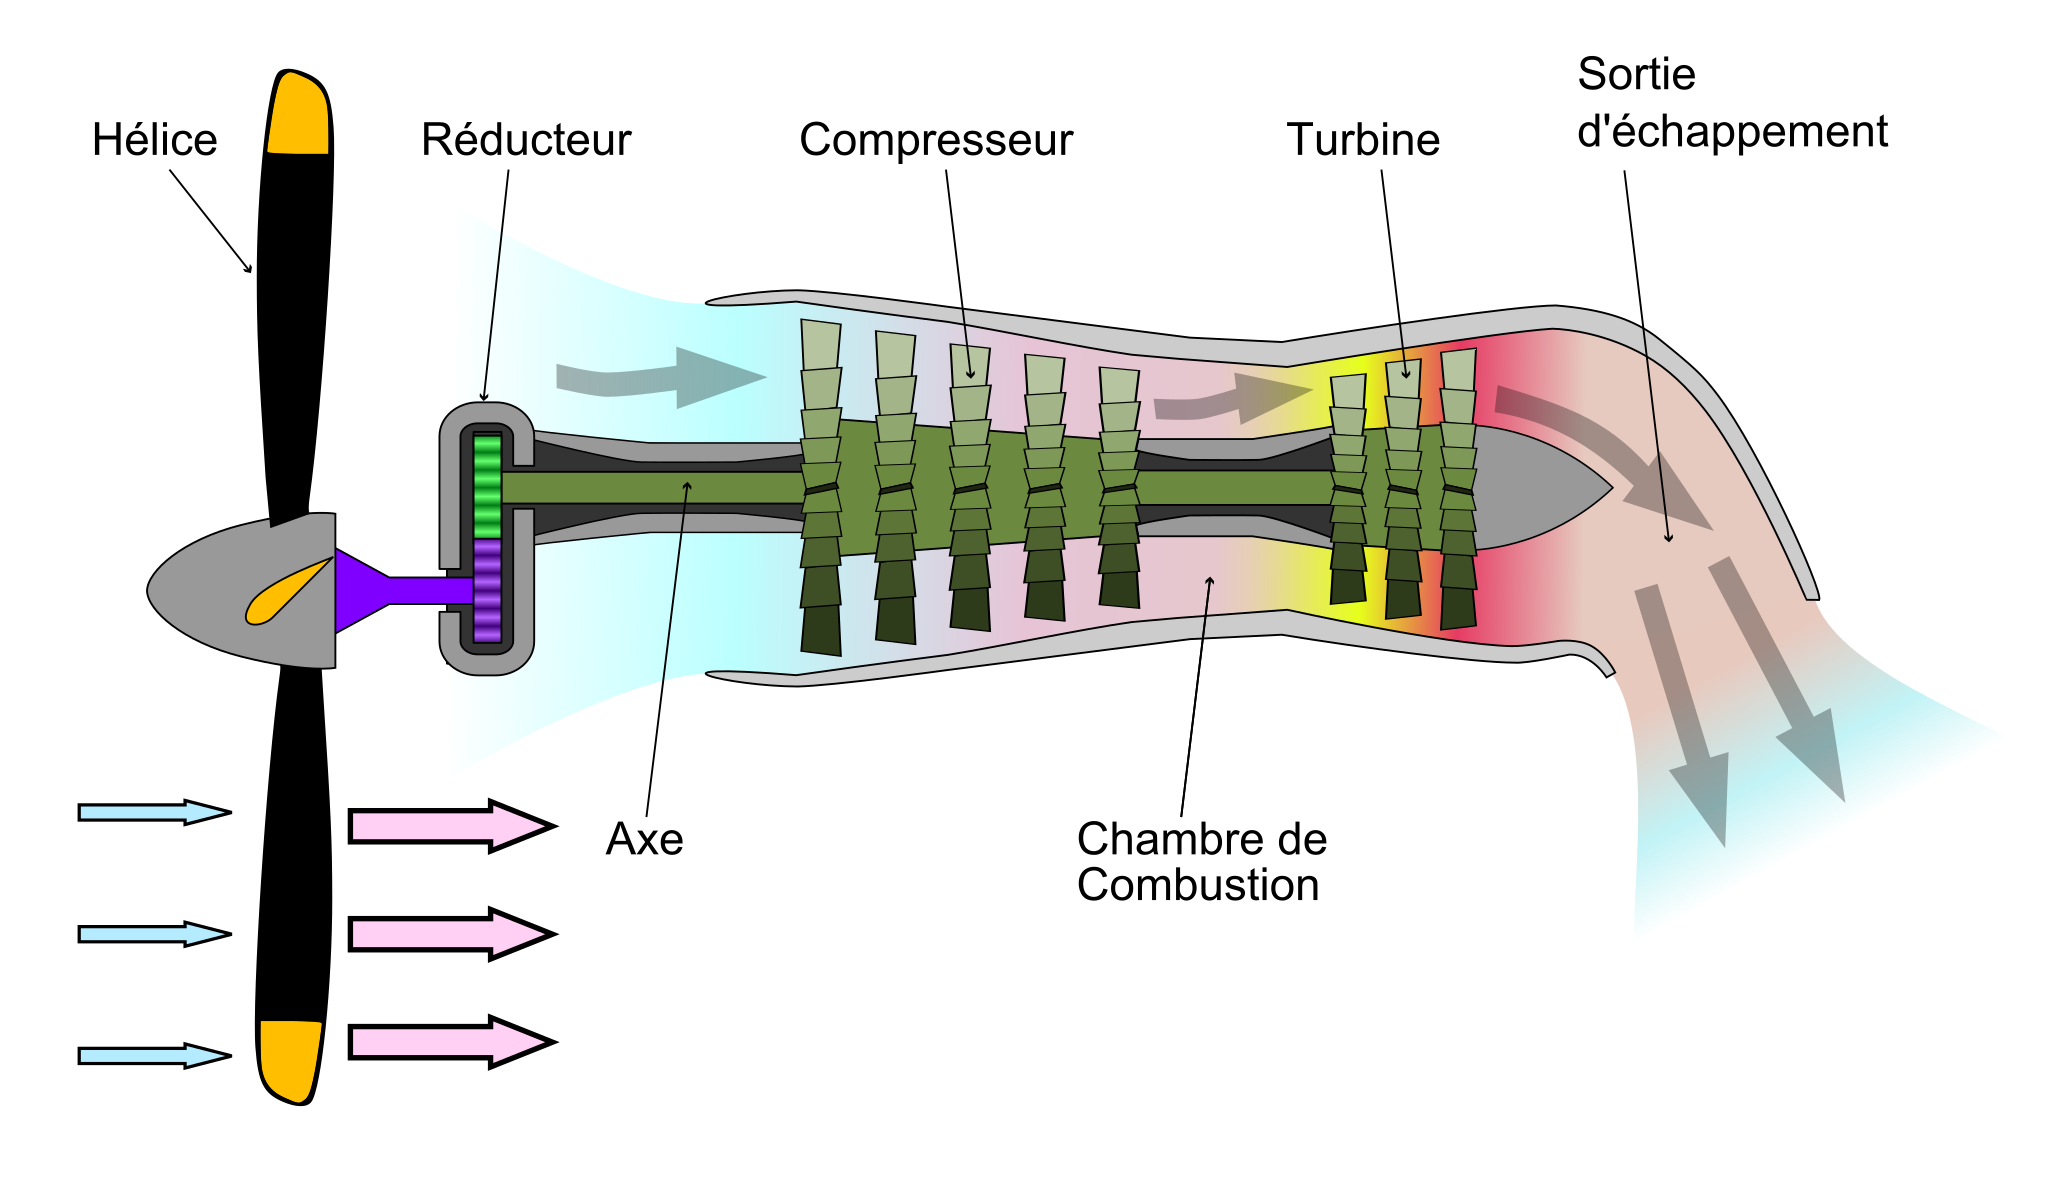
\includegraphics[width=0.75\textwidth]{01-EtudeAeronefs/img/turbomachines/turbopropulseur.pdf}
  	\legende{Schéma d'un turbopropulseur}{img:turbopropulseur}
	\end{figure}	
	
	\subsection{Hélices et moteurs}
	
	\subsection{Propulseurs à réaction}
		\subsubsection{Turboréacteurs}
		
		\begin{figure}[H]
  		\centering
    		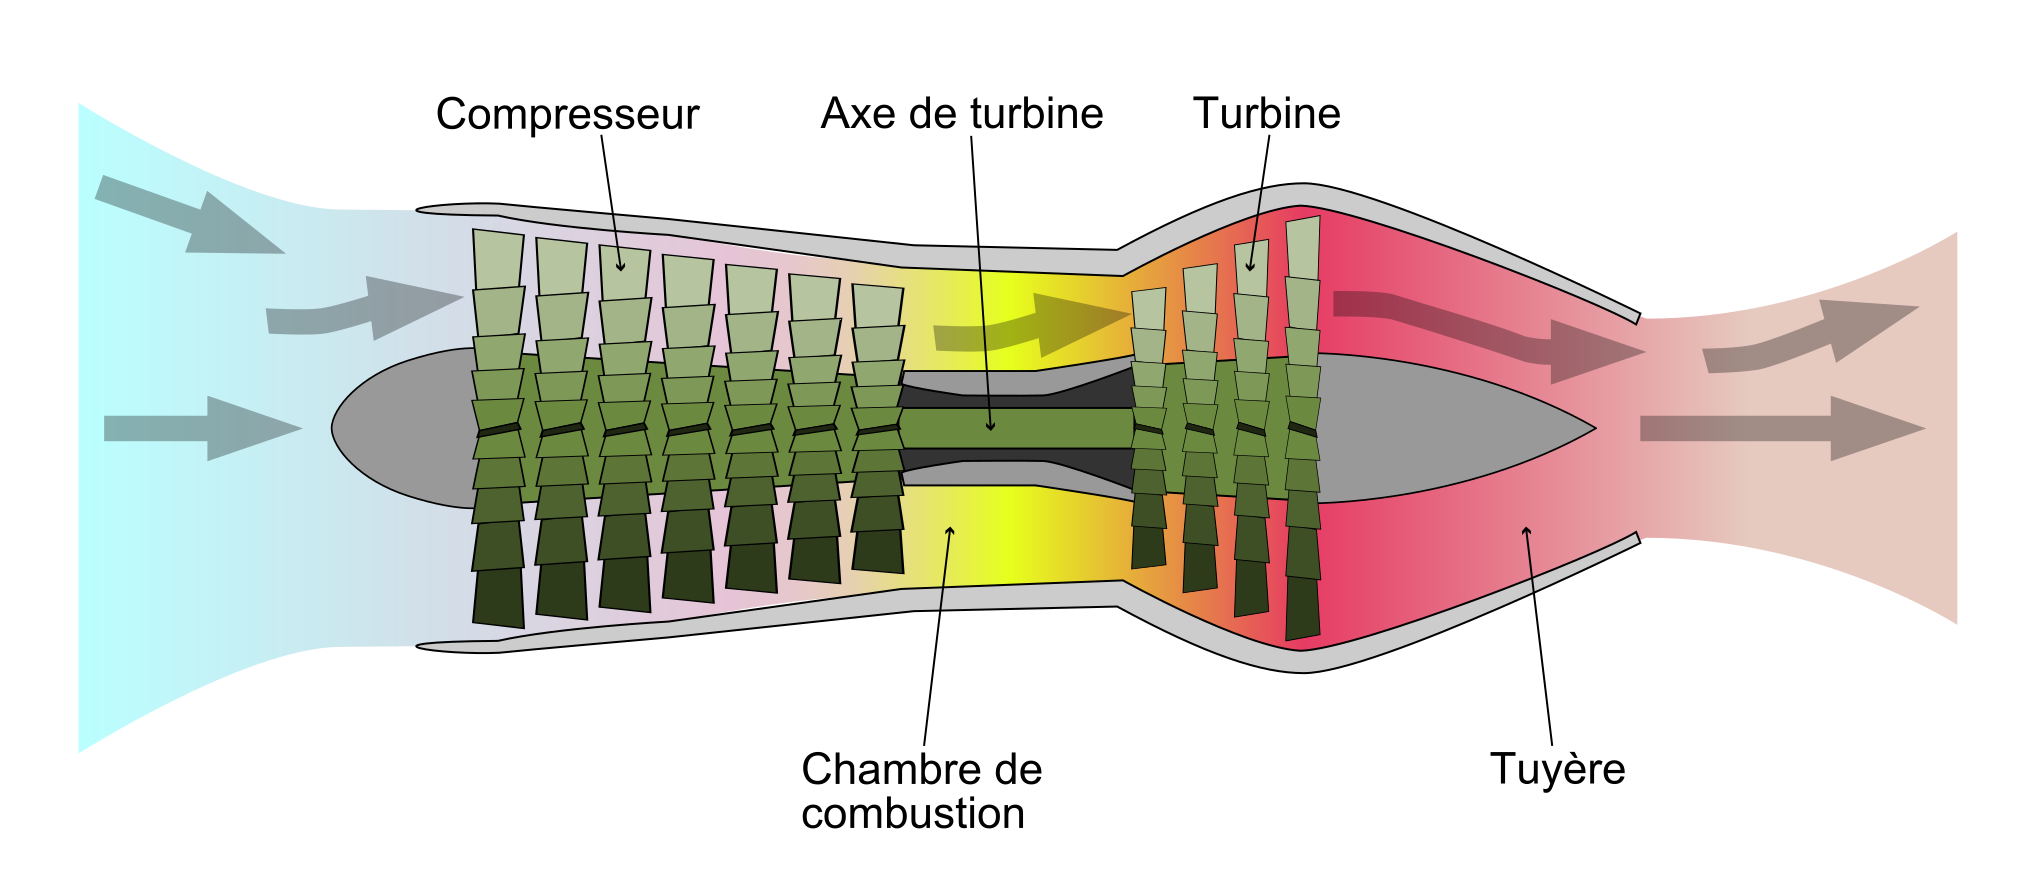
\includegraphics[width=0.75\textwidth]{01-EtudeAeronefs/img/turbomachines/turboreacteur-simpleFlux.pdf}
  		\legende{Schéma d'un turboréacteurs simple flux}{img:turboreacteur-simpleFlux}
		\end{figure}	
	
		\begin{figure}[H]
  		\centering
    		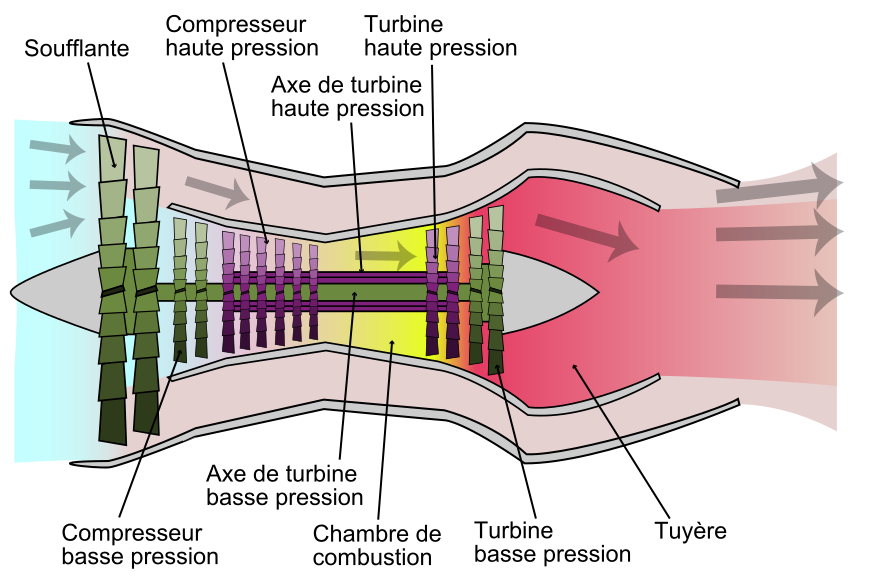
\includegraphics[width=0.75\textwidth]{01-EtudeAeronefs/img/turbomachines/turboreacteur-doubeFlux.pdf}
  		\legende{Schéma d'un turboréacteurs double flux}{img:turboreacteur-doubeFlux}
		\end{figure}	
	
		\subsubsection{Statoréacteurs}
	
		\subsubsection{Moteurs fusées}
		
	\subsection{Contraintes liées au développement durable}
